\documentclass[titlepage]{scrartcl}

% German support
\usepackage[utf8]{inputenc}
\usepackage[ngerman]{babel}
\usepackage[T1]{fontenc}

%\usepackage[english]{babel}

\usepackage{graphicx}
\usepackage[dvipsnames]{xcolor}
\usepackage{float}
\usepackage{placeins}

\usepackage{enumitem}

\usepackage{caption}
\usepackage{subcaption}

\usepackage[autostyle]{csquotes}

% Make citations clickable
\usepackage{hyperref}

\usepackage{url}


\usepackage{listings}

\renewcommand{\lstlistingname}{Code}
\renewcommand{\lstlistlistingname}{Quellcodeausschnitte}

% Define TypeScript as language for listings
\lstdefinelanguage{TypeScript}{
	keywords={
		typeof, new, true, false,
		function, class, this, null,
		var, let, const, in, is,
		async, instanceof, private,
		public, readonly, constructor
	},
	keywordstyle=\color{blue}\bfseries,
	otherkeywords={% Operators
		=>
	},
	ndkeywords={
		return, if, while, do, else, catch,
		switch, case, break, export, boolean,
		throw, implements, import, await
	},
	ndkeywordstyle=\color{violet}\bfseries,
	identifierstyle=\color{black},
	sensitive=false,
	comment=[l]{//},
	morecomment=[s]{/*}{*/},
	commentstyle=\color{ForestGreen},
	stringstyle=\color{red},
	morestring=[b]',
	morestring=[b]",
	morestring=[b]`
}

\lstdefinelanguage{CSharp}{
	keywords={
		abstract, event, new, struct, var,
		as, explicit, null, switch,
		base, extern, object, this,
		bool, false, operator, throw,
		break, finally, out, true,
		byte, fixed, override, try,
		case, float, params, typeof,
		catch, for, private, uint,
		char, foreach, protected, ulong,
		checked, goto, public, unchecked,
		class, if, readonly, unsafe,
		const, implicit, ref, ushort,
		continue, in, return, using,
		decimal, int, sbyte, virtual,
		default, interface, sealed, volatile,
		delegate, internal, short, void,
		do, is, sizeof, while,
		double, lock, stackalloc,
		else, long, static,
		enum, namespace, string
	},
	keywordstyle=\color{blue}\bfseries,
	otherkeywords={% Operators
		=>
	},
	identifierstyle=\color{black}\bfseries,
	sensitive=false,
	comment=[l]{//},
	morecomment=[s]{/*}{*/},
	commentstyle=\color{ForestGreen},
	stringstyle=\color{red},
	morestring=[b]',
	morestring=[b]",
	morestring=[b]`
}

%define colors for json
\colorlet{punct}{red!60!black}
\definecolor{delim}{RGB}{20,105,176}
\colorlet{numb}{magenta!60!black}

\lstdefinelanguage{json}{
    literate=
     *{0}{{{\color{numb}0}}}{1}
      {1}{{{\color{numb}1}}}{1}
      {2}{{{\color{numb}2}}}{1}
      {3}{{{\color{numb}3}}}{1}
      {4}{{{\color{numb}4}}}{1}
      {5}{{{\color{numb}5}}}{1}
      {6}{{{\color{numb}6}}}{1}
      {7}{{{\color{numb}7}}}{1}
      {8}{{{\color{numb}8}}}{1}
      {9}{{{\color{numb}9}}}{1}
      {:}{{{\color{punct}{:}}}}{1}
      {,}{{{\color{punct}{,}}}}{1}
      {\{}{{{\color{delim}{\{}}}}{1}
      {\}}{{{\color{delim}{\}}}}}{1}
      {[}{{{\color{delim}{[}}}}{1}
      {]}{{{\color{delim}{]}}}}{1},
}

\definecolor{background}{HTML}{EEEEEE}

\lstset{
	basicstyle=\ttfamily\footnotesize,
	frame=lines,
	captionpos=b,
	%rulecolor=\color{blue!80!black},
	inputencoding=utf8,
	tabsize=2,
	numbersep=5pt,
    showstringspaces=false,
	extendedchars=true,
	numbers=left,
	breaklines=true,
	backgroundcolor=\color{background},
}

\lstdefinestyle{sharpc}{
	language=CSharp,
	escapechar=`
}


\newenvironment{codeblock}{%
	\bigskip
	%\begin{fullwidth}[width=\linewidth+4cm]
		\noindent\begin{minipage}{\linewidth}%
}
			% Code
{%
		\end{minipage}
	%\end{fullwidth}%
}




\bibliographystyle{plain}


\begin{document}
	\titlehead{Technische Hochschule Deggendorf}
	\subject{Documentation}
	\title{AR Sensor Visualisation}
	%\subtitle{}
	\author{Michael Mican\\Matrikel-Nr.: 692390 \and Maximilian Seitz\\Matrikel-Nr. 692807}
	%\date{}
	\publishers{Technische Hochschule Deggendorf\\Advisor: Prof. Dr. Peter Faber}
	
	\maketitle
	
	\tableofcontents
	\pagebreak
	
	\section{Einleitung}

\begin{itemize}
	\item Visuelles für den Menschen am wichtigsten zur info aufnahme
	\begin{itemize}
		\item Schon der neandertaler musste in bruchteilen einer sekunde die information über den Anstürmenden Leoparden verarbeiten können
	\end{itemize}
	
	\item => AR/MX wird immer cooler
	\item Erreicht auch konsumenten markt: Siehe Nintendo Mariokart AR
	\item Allgemeine vorteile von AR
	\item AR auch im Enterprise bereich sinnvoll zu visualisierung von Daten
	\begin{itemize}
		\item Weniger abstrakt/Daten werden verständlicher/greifbarer
	\end{itemize}
	
	\item -> Beispiel überletung
\end{itemize}
	\section{Entwurf}
Für die Realisation und das Erreichen des Ziels musste ein konkretes Vorgehen und ein grundsätzliche Architektur definiert werden. Hierfür spielten verschiedene Faktoren eine Rolle, welche im nachfolgenden beleuchtet werden.

\subsection{Allgemeiner Aufbau}
Da die Applikation von Grund auf entwickelt wird, wird der Allgemeine Aufbau von den beiden Entwicklern Maximilian Seitz und Michael Mican definiert. Der betreuende Professor Prof. Dr. Peter Faber fungiert während der Entwicklung als Project Owner.

\subsubsection{Projekt Vorgaben}
Das Kernziel bestand in der Visualisierung von Vektoren im dreidimensionalen Raum, welche den gemessenen magnetnischen Fluss eine flüssigen Metalls in Echtzeit auf eine verschlossene Kokille zu projizieren. Dies soll möglichst unkompliziert und Zugänglich ermöglicht werden, um auch kurzfristig ohne großen Aufwand Besuchern und Gästen eine Benutzung zu ermöglichen. Aus diesem Grund wird eine Webbasierte Lösung umgesetzt, da so in der Theorie nur eine Webseite mit dem Smartphone besucht werden muss um die Applikation zu benutzen. In vorangehenden ähnlichen Projekten wurde deutlich, dass Übersichtlichkeit hierbei eine große Rolle spielt. Zur Lösung des Problems soll eine frei Bewegliche ebene mit definierbarer dicke im Vektorfeld bewegt werden können um so nur nach einem Ausschnitt der Daten intuitiv Filtern zu können. Da die Daten direkt vor Ort gemessen und Sicherheitsrelevant besitzen soll es möglich sein die Daten in einem lokalen Netzwerk zu hosten um eine grundlegende IT - Sicherheit zu gewährleisten. Hierbei treten jedoch unter Berücksichtigung der anderen Vorgaben Probleme auf.


%\begin{itemize}
%	\item Was will man visualiseren?
%	\begin{itemize}
%		\item Magnetischerfluss von Flüssigem metall in Kokille
%		\item Soll dabei helfen die einlaufgeschwindigkeit zu regulieren
%	\end{itemize}
%	
%	\item Geschlossenes netzwerk
%	\begin{itemize}
%		\item Kein Internet zugriff
%	\end{itemize}
%	
%	\item Möglichkeit der filterung der visuellen Ergebnisse
%	\item Soll auf Handy ohne Einstellungen laufen\\
%		("Einfach auf website gehen und LETS GOOOOOO")
%\end{itemize}


\subsubsection{Probleme und Abweichungen von den Vorgaben}
Seit einigen Jahren können sogenannte \grqq Powerful Features\grqq\space nurnoch von Seiten mit \grqq Secure origin\grqq , also zertifizierte HTTPS Seiten, genutzt werden. Diese Entscheidung fiel auf Grundlage technischer Fortschritte, die es aus sicherheitsrelevanter Sicht nicht mehr vertretbar machte Funktionen wie Beispielsweise Geräteposition und Kamera von klassischen nicht zertifizierten HTTP Seiten zu ermöglichen (vgl. The Chromium Projects \cite{CameraHTTPSOnly}). Die Datenübermittlung, welche von HTTPS genutzt wird, macht es Angreifern schwerer solche kritische Daten abzugreifen. Somit ist es erforderlich eine HTTPS-Webseite für die Applikation zu nutzen. Daher wird die Frontend Seite über Github distributiert, wodurch sie ein HTTPS Zertifikat einer anerkannten Zertifizierungsstelle erwirbt. Diesem vertrauen Webbrowser Standardmäßig wodurch eine Manuelle Einstellung am Endgerät nicht getätigt werden muss.\\
Dieses vorgehen führt zu einem weiterem Problem. Seit Anfang 2020 ermöglicht es Google Chrome standardmäßig nicht mehr HTTP Quellen auf einer HTTPS-Seite zu benutzen (vgl. Chromium Blog \cite{MixedSourcesPolicy}). Unter Berücksichtigung der Vorgabe des Project Owners, welche die Nutzung eines Datenservers ohne Internetzugang im lokalen Netzwerk vorsieht, ist eine Einstellung am Endgerät unumgänglich. Hierfür gibt es zwei möglichkeiten.\\
Einerseits kann, um einen unzertifizierten HTTP Datenserver im lokalen Netzwerk benutzen zu können, die Einstellung \grqq Allow unsecure content\grqq\space in den Browser Einstellungen auf \grqq Allow\grqq\space gesetzt werden. Hierdurch wird die Mixed Content policy ignoriert und HTTP Quellen können auch auf der Seite benutzt werden. In Chrome Desktop kann diese Option in den Webseiteneinstellungen gefunden werden. Auf einem Smarphone hingegen muss hierfür der interne Settings link \verb|"chrome://flags/#unsafely-treat-insecure-origin-as-secure"| genutzt werden (siehe Abbildung \ref{fig:insecureOriginsSettings}).\\
Die zweite Möglichkeit das Problem zu lösen erfordert eine eigene definierte HTTPS Zertifizierung des Datenservers. Da diese Zertifizierung nicht via Internet geschehen kann muss hierfür ein eigenes benutzerdefiniertes Zertifikat angelegt und am Endgerät, welches die Website aufruft, als bekanntes Zertifikat installiert werden.\\ 
Nach Abstimmung mit dem Project Owner wird das Problem bis auf weiteres bei der Entwicklung nicht berücksichtigt. Stattdessen wird sowohl das Frontend als auch das backend mit Simulierten Daten im Internet mit validen HTTPS zertifikaten gehostet.

\begin{figure}
	\centering
	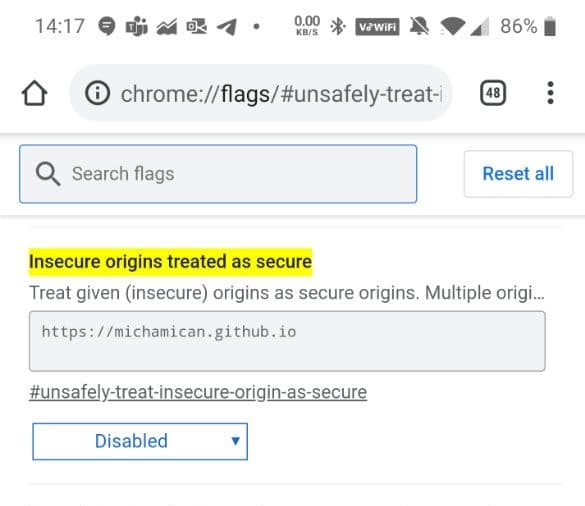
\includegraphics[width=.75\linewidth]{images/InsecureOriginsSettings}
	\caption{Allow insecure origin in Chrome mobile}
	\label{fig:insecureOriginsSettings}
\end{figure}

%\begin{itemize}
%	\item HTTPS erforderlich für kamera
%	\begin{itemize}
%		\item Lokaler Host Server braucht SSL zertifikat - Manuelle trustung des Zertifikats am handy unumgänglich
%	\end{itemize}
%	
%	\item HTTPS oder unsecured source Einstellung für backend kommunikation erforderlich
%	\item=> Für Beispielzwecke beides HTTPS via Internet
%\end{itemize}


\subsubsection{Komponenten}
\label{section:Komponenten}

Um Komponenten austauschbar zu machen, und Wiederverwendung davon zu
ermöglichen, wird eine Architektur mit einem Frontend und Backend
umgesetzt. Dabei übernimmt das Frontend die Visualisierung der Daten,
in der Form einer Website, die die Daten, welche Angezeigt werden,
von einem Server einholt, der das Backend bildet.

Dabei werden die Aufgaben so verteilt, dass das Frontend unabhängig
vom genauen Anwendungsgebiet ist, zu welchem ihm das Backend alle
Informationen über eine API zur Verfügung stellt.

Um dies zu ermöglichen, wird die Funktionalität auf ihre abstrakten
Bestandteile reduziert, die dann vom Frontend unterstützt wird.
Diese Teile sind die Anzeige von einem Vektorfeld, und einem
3D-Modell der Umgebung, projiziert auf die echte Welt, durch die
Kamera. Synchronisierung findet hierzu über einen AR-Marker statt.
Diese Funktionalitäten sind die Voraussetzung, welche jedoch
erweitert werden, um das Nutzen der Anwendung zu erleichtern.
Jegliche solche Änderungen sind in Kapitel \ref{section:Frontend}
beschrieben. Die vorausgesetzten Kommunikationsschnittstellen werden
in Kapitel \ref{section:Backend} genauer beschrieben.

Durch diese Architektur, ist ein Austausch des Backends möglich,
was Visualisierung anderer Daten erlaubt. Diese Datenquellen können
beispielsweise Luftströme um ein Objekt anzeigen, zuvor aufgenommene
Daten wiedergeben, oder Abwärme simulieren. Das Frontend ist dazu
fähig auch solche Daten, mit den selben mitteln, an zu zeigen.

%\begin{itemize}
%	\item Backend vs. Frontend
%	\begin{itemize}
%		\item Frontend: AR visualisierung (allgemein)
%		\item Backend: Implementierungs spezifizierung
%		\item ziel: Frontend kann mit verschiedenen Backends genutzt werden
%	\end{itemize}
%\end{itemize}


\subsection{Visualisierung/Frontend}
\label{section:Frontend}
\FloatBarrier

Für das Anzeigen von Daten wird eine Website entwickelt, welche
für Smartphones optimiert wird. Diese Website bildet das, in Kapitel
\ref{section:Komponenten} eingeführte, Frontend der Anwendung.
Die hier umgesetzte Website fungiert als portable, und dynamisch
auslieferbare Applikation, die von einem Webservice, dem Backend,
Daten anfordert, um diese an zu zeigen.

\begin{figure}
	\centering
	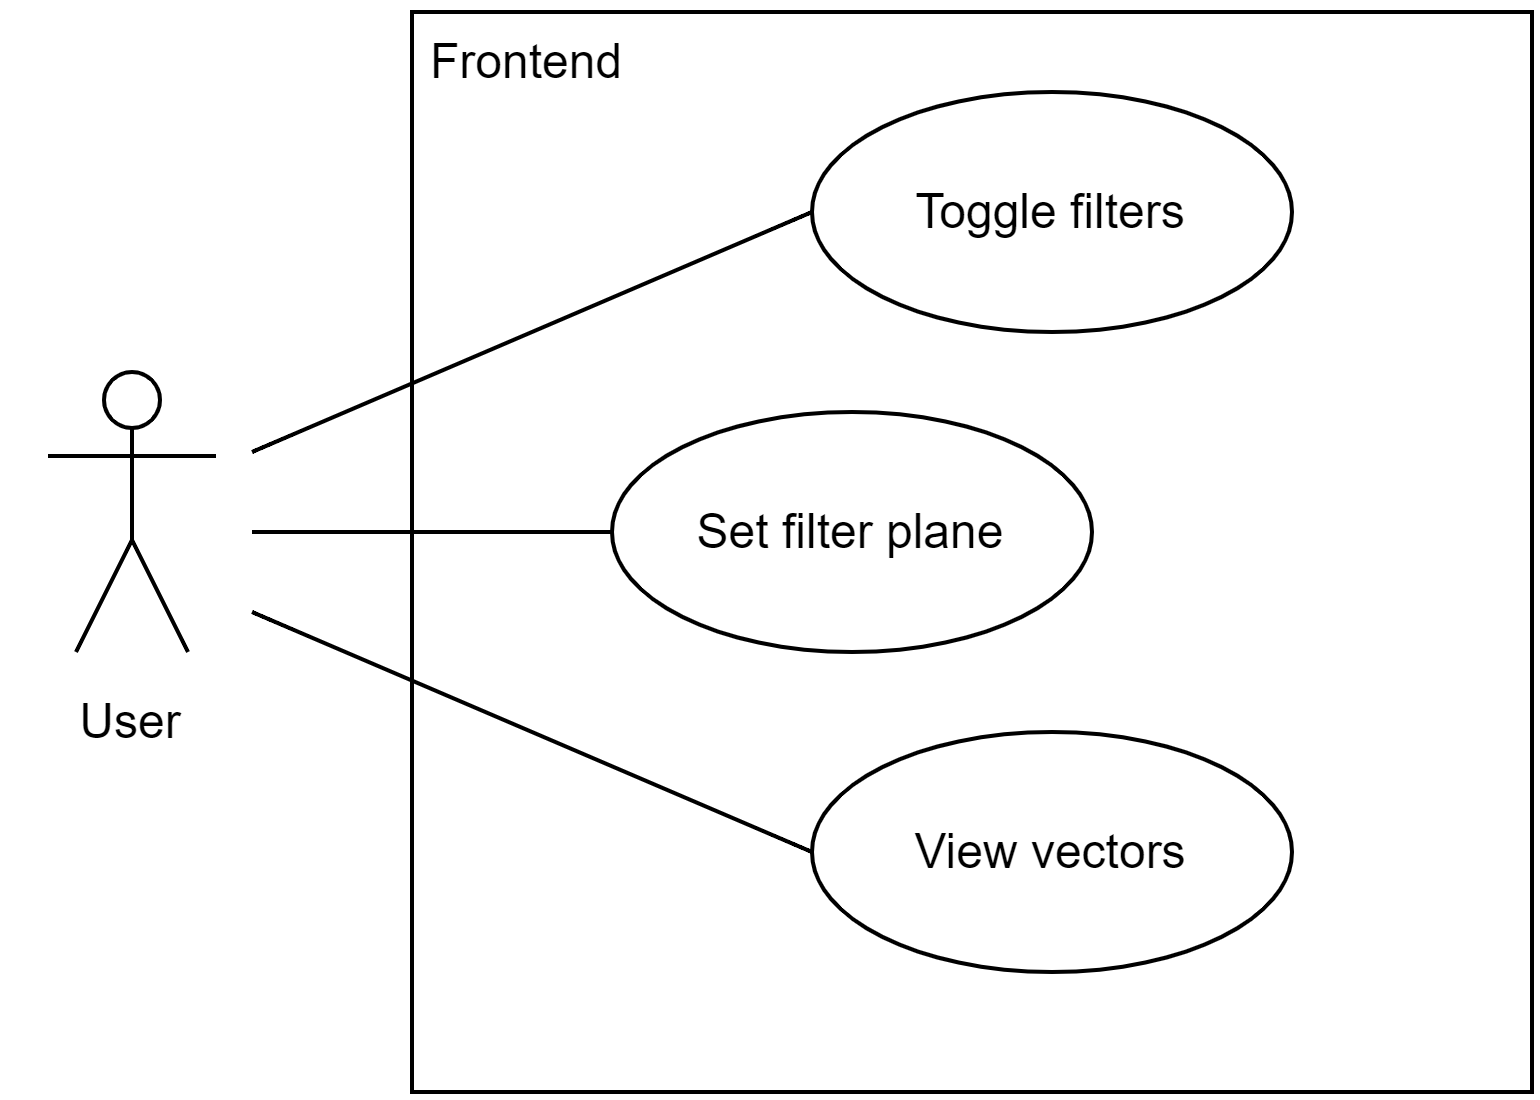
\includegraphics[width=.6\linewidth]{images/frontend/UseCases}
	\caption{Frontend use cases.}
	\label{fig:frontendUseCase}
\end{figure}

Abbildung \ref{fig:frontendUseCase} zeigt die Nutzungsmöglichkeiten
des Frontends. Es werden 3D-Vektoren als Pfeile dargestellt,
die abhängig von ihrer Länge eingefärbt sind. Dabei werden
Änderungen der Daten, in regelmäßigen abständen, angenommen. Diese
Änderungen werden abgefragt, jedoch liegt dabei der Fokus darin, die
Pfeile für den Nutzer erkennbar dar zu stellen, statt möglichst
Echtzeitdaten zu nutzen. Es wird zudem erlaubt die Vektoren auf eine
Örtlich begrenzte Gruppe ein zu schränken, wodurch nur diese
dargestellt wird. Um den Vektoren visuelle Referenzpunkte zu geben,
wird ein Grundgerüst geladen und angezeigt. Dieses Gerüst ist ein
unveränderliches 3D-Objekt, um das die Pfeile sich befinden.
Diese Szene wird über einen Kamerastream gezeichnet. Dabei wird
aus dem Bild ein, vom Backend definierter, Marker gesucht,
von welchem eine 3D-Position berechnet wird. Diese Position wird
genutzt, um die 3D-Szene zu positionieren, und sie in der echten
Welt zu ankern. Dies lässt die 3D-Szene als Erweiterung der echten
Welt erscheinen, und macht sie zur so genannten \grqq Augmented
Reality\grqq\space (vgl. AR.js Documentation \cite{ARjsDoc}).

Um virtuelle Objekte performant darzustellen, wird OpenGL genutzt.
Der Zugriff darauf wird von der JavaScript Bibliothek
\grqq Three.js\grqq\space übernommen. Als vereinheitlichte
Schnittstelle zur Echten Welt, wird \grqq AR.js\grqq , als
Erweiterung von \grqq Three.js\grqq\space genutzt.
\grqq AR.js\grqq\space steuert den Zugriff auf die Kamera des
Endgerätes, und erkennt darin den geladenen Marker. Für diesen
Marker wird ein virtuelles Gegenstück erzeugt, welches die
gleiche relative Größe und Position zur virtuellen Kamera hat,
wie dar physische Marker, zur physischen Kamera.

\begin{figure}
	\centering
	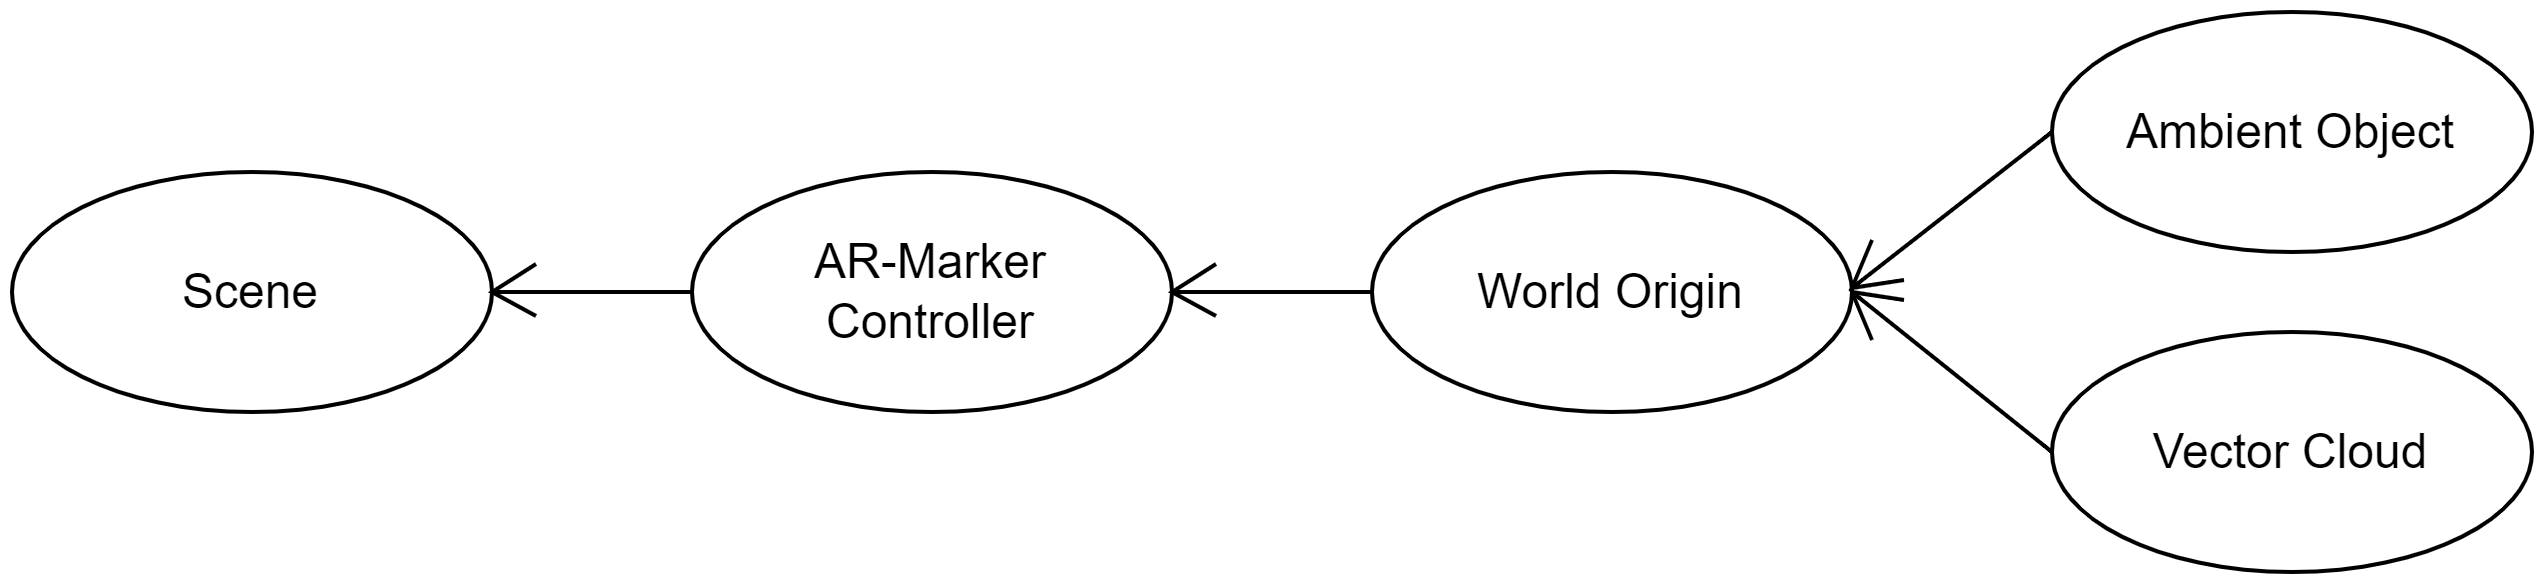
\includegraphics[width=1\linewidth]{images/frontend/SceneTree}
	\caption{Szenen-Baum des Frontends}
	\label{fig:SceneTree}
\end{figure}

Abbildung \ref{fig:SceneTree} zeigt den Szenen-Baum, der
Beschreibt wie die Objekte im der Szene voneinander beeinflusst
werden. Jedes Objekt erbt von seinem Vorfahren die Position und
Skalierung. Objekte sind hier nicht dringend mit einer graphischen
Darstellung verbunden. Solche Objekte werden \grqq Gruppen\grqq\space
genannt. Die \grqq Szene\grqq\space ist eine Gruppe, deren Nachkommen
angezeigt werden. Der \grqq AR-Marker Controller\grqq\space ist die
Gruppe, die von \grqq AR.js\grqq\space an die Kamera angepasst wird.
Alle Objekte, die teil der AR Darstellung sind, sind Nachkommen dieser
Gruppe. Da der Marker in Größe und Position, in Abhängigkeit des
logischen Koordinatenursprungs der echten Welt variiert, wird die
Gruppe \grqq World Origin\grqq\space angelegt. Bei einer Verschiebung
des Markers im Versuchsumfeld, kann der \grqq World Origin\grqq\space
gegenläufig, mit dem gleichen Betrag, verschoben werden, um dies zu
korrigieren. Diese Gruppe hat die angezeigten Objekte als Kinder.
Das ist einerseits das \grqq Ambient Object\grqq , welches zur
Orientierungshilfe dient, und andererseits eine \grqq Vector
Cloud\grqq , was eine Menge an Pfeil-Objekten ist, die angepasst
werden, um die Vektoren darzustellen, ohne regelmäßig neue Objekte
zu erstellen und zerstören.

%\begin{itemize}
%	\item Abbildung \ref{fig:frontendUseCase} zeigt
%		die Möglichkeiten des Frontends.
%	\begin{itemize}
%		\item Filtern
%		\item Anzeigen
%	\end{itemize}
%	
%	\item Three.js + AR.js
%	\begin{itemize}
%		\item OpenGL
%	\end{itemize}
%
%	\item Auswahl von Filter-Parametern
%	\item Object-Tree:
%	\begin{itemize}
%		\item Marker-Origin (wird von AR.js verschoben -> auf Marker in Quelle)
%		\begin{itemize}
%			\item Welt-Origin (korrigiert Marker verschiebung+rotation+skalierung von welt-origin)
%			\begin{itemize}				
%				\item Kokille Modell
%				\item Pfeile (10000 * ArrowHelper)
%				\item Filter-Box
%			\end{itemize}
%		\end{itemize}
%	\end{itemize}
%\end{itemize}



\subsection{Daten Bereitstellung/Backend}
\label{section:Backend}

Zur Bereitstellung der Daten wird eine REST API implementiert.
Über diese API kann das Frontend alle Usecase spezifischen Daten
abrufen (siehe Abbildung \ref{fig:backendUseCase}). Somit kann dasselbe Frontend durch eine einfach Änderung der API-URL an mehren
Orten verwendet werden. Alle Antworten der API sind in JSON codiert,
da JSON besser für dynamische Webapplikationen und einfachen
Datentransfer geeignet ist als andere ähnliche Datenformate wie
XML (vgl. Šimec \cite{comparisonJsonXml}). Die Vektordaten werden
als Array zurückgegeben. Jedes Vektorobjekt besitzt jeweils eine
x, y, z, xVec, yVec und zVec Property (Siehe Code \ref{code:VecJSON}).
Sie definieren den Fußpunkt des Vektors (x, y, z) und die Richtung
des Vektors (xVec, yVec, zVec).

\begin{codeblock}
	\begin{lstlisting}[
		language=json,
		caption={Aufbau der Vektordaten JSON},
		label={code:VecJSON}
	]
[
	{
		"x": float,
		"y": float,
		"z": float,
		"xVec": float,
		"yVec": float,
		"zVec": float
	}
]
	\end{lstlisting}
\end{codeblock}

Grundsätzlich müssen 2 wichtige Endpunkte implementiert werden und ein Endpunkt zur Datenbereitstellung verfügbar gemacht werden.
Der Datenbereitstellungs-Endpunkt hostet die eingangs erwähnten Usecase spezifischen statischen Dateien. Hierzu zählen die modellspezifischen Daten, welche die visuelle Representation und Texturierung der Kokille darstellen, die Settings und Parameter für die Kamera und das Markerpattern und Informationen zu Positionierung und Skalierung der echten Kokille relativ zum Marker.\\
Die beiden anderen Endpunkte werden für die gemessenen Vektordaten verwendet. Sie bieten die Möglichkeit über eine GET Schnittstelle die Vektordaten zu holen und über eine weitere GET Schnittstelle die Metadaten dieser Vektoren, wie die Anzahl und die jeweiligen min und max x,y und z werte der Vektoren, zu beziehen. Darüber hinaus ist es möglich bei der Datenabfrage über Query Parameter einen Einheitsvektor und eine Distanz mitzugeben, welche eine Filterebene definiert, sodass nur Vektoren innerhalb der definierten Distanz von dieser Filterebene zurückgegeben werden.\\
Diese Endpunkte müssen von anderen Seiten und Domänen abgefragt werden können. Aufgrund von Cross-Origin Resource Sharing Policies (CORS) ist hierfür ein spezielles Vorgehen erforderlich. Der Client sendet bei seiner Anfrage im \grqq Origin\grqq\space Header seine Domäne mit. Der Server muss diese Domäne akzeptieren und in seiner Antwort den \grqq Access-Control-Allow-Origin\grqq\space Header mit der jeweiligen Domäne oder einem \grqq *\grqq\space befüllen (vgl. Kesteren \cite{van2014cross}). Der hier implementierte Backend-Server gibt immer einen \grqq Access-Control-Allow-Origin\grqq\space Header mit dem Wert \grqq *\grqq\space zurück, wodurch jegliche Seiten und Domänen die Daten akquirieren können. Dies kann aber im Anwendungsfall aus sicherheitstechnischen Gründen geändert werden müssen.

\begin{figure}
	\centering
	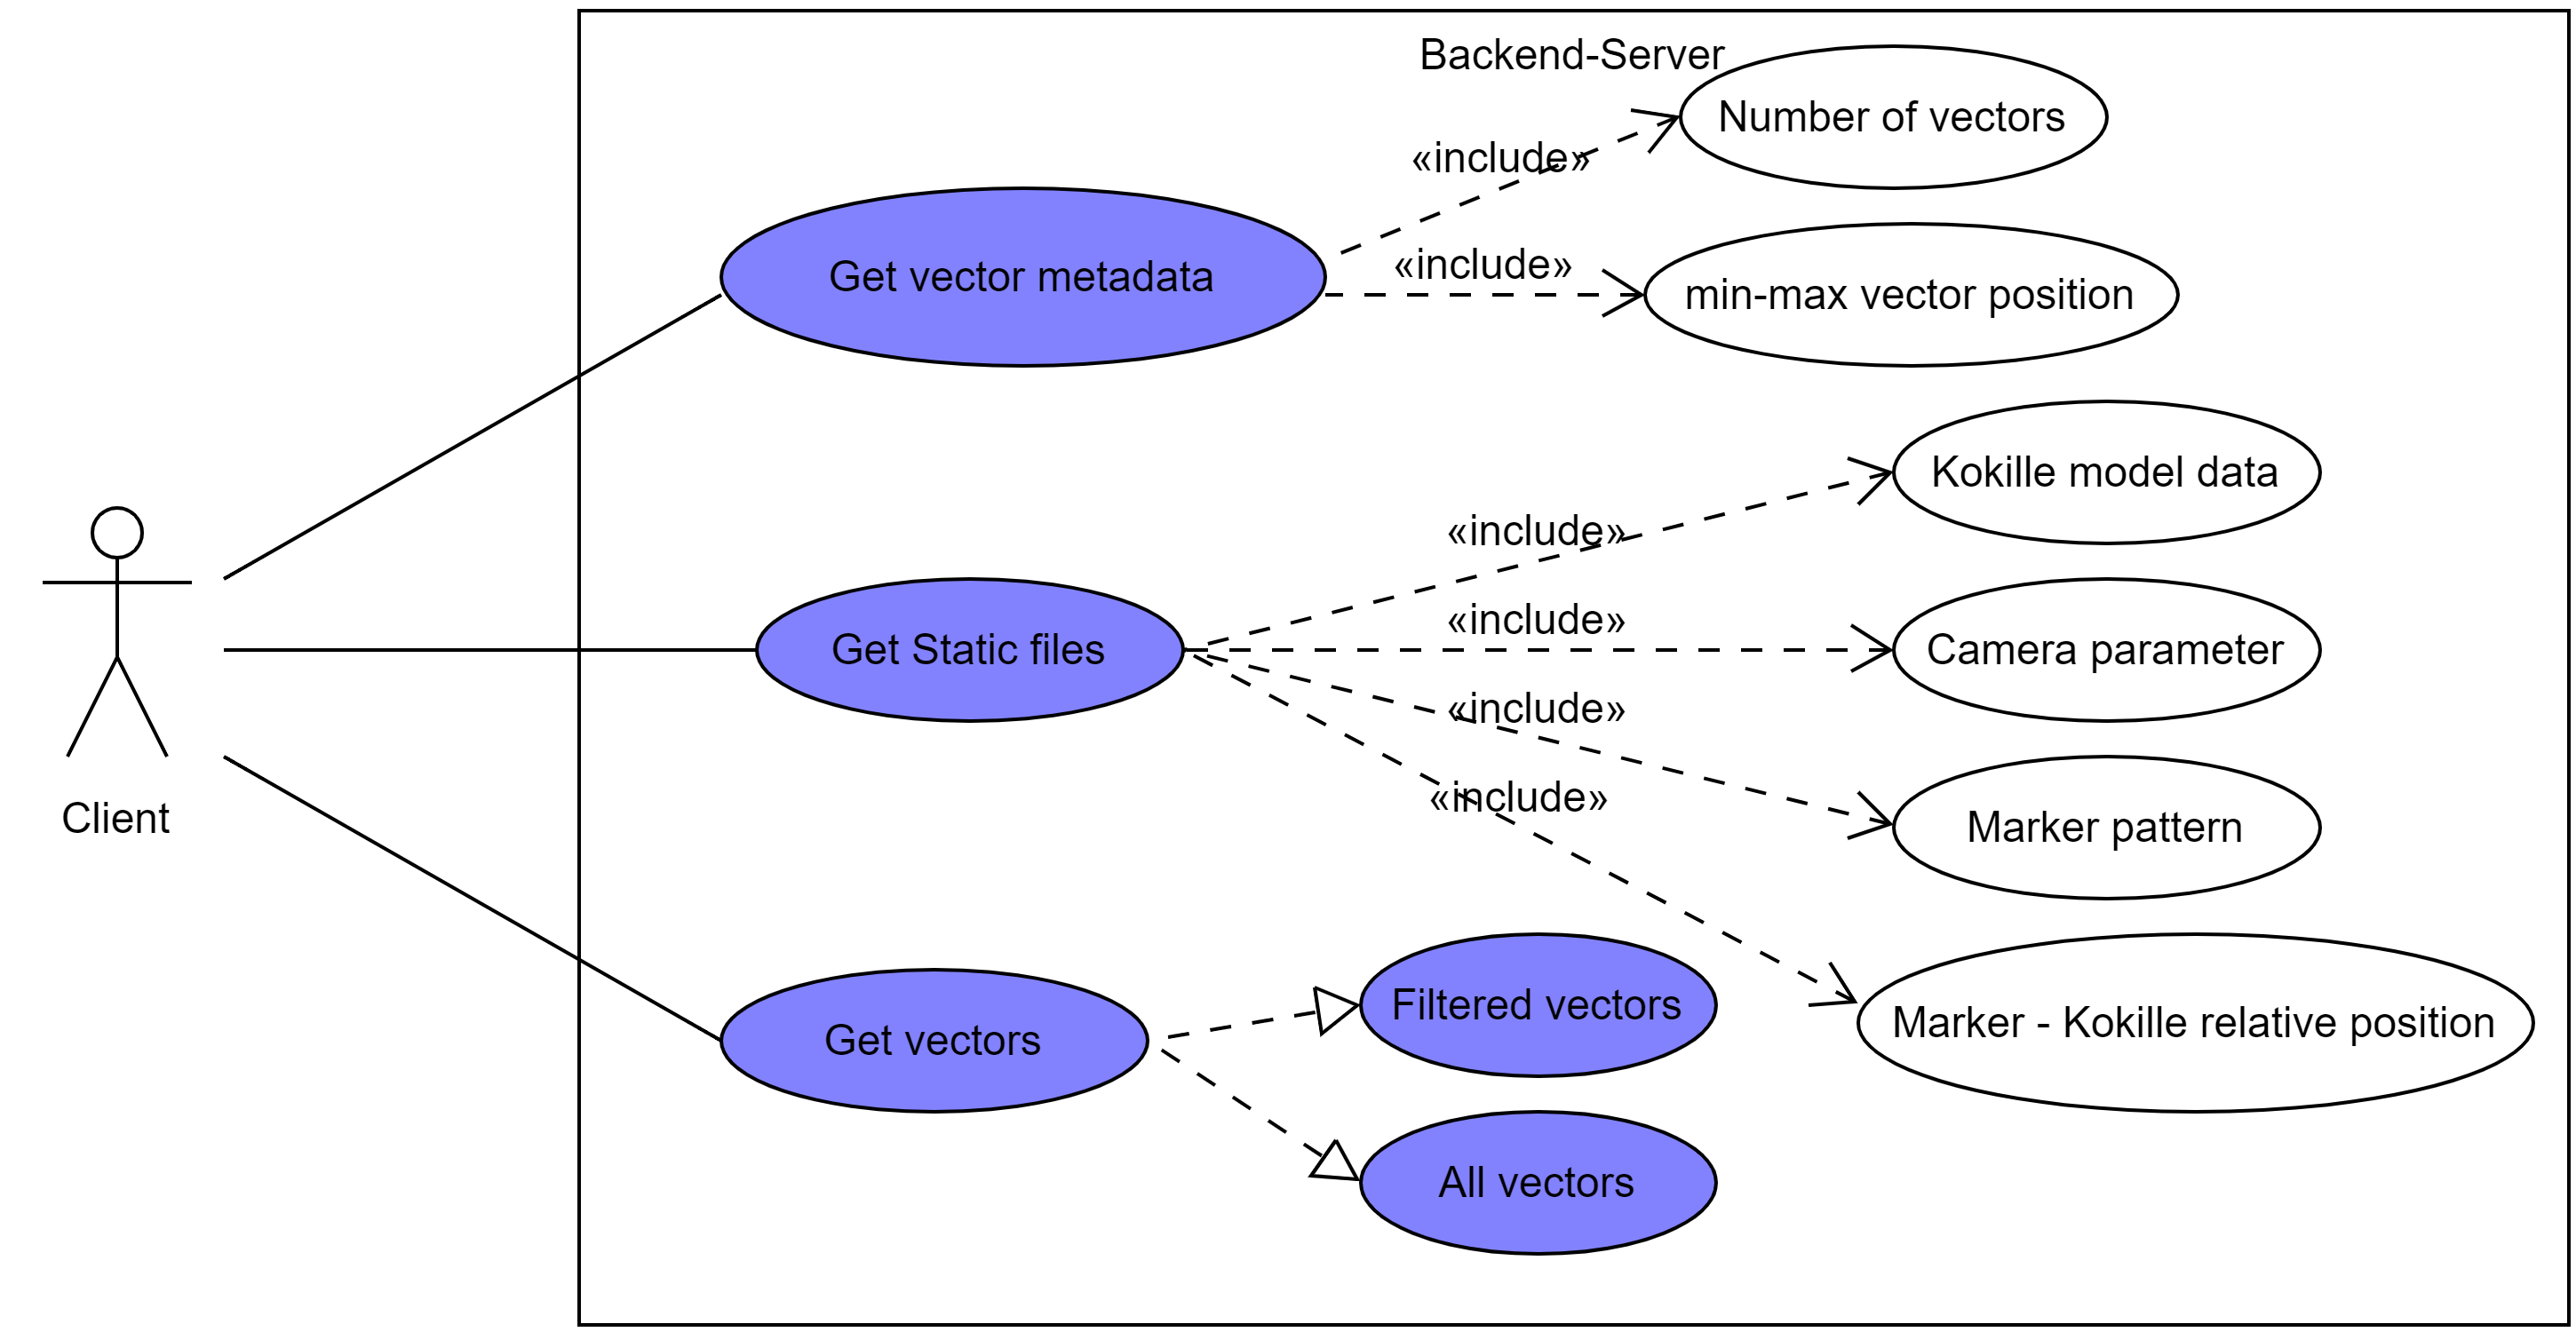
\includegraphics[width=1\linewidth]{images/backend/APIUseCases}
	\caption{API use cases.}
	\label{fig:backendUseCase}
\end{figure}


%\begin{enumerate}
%	\item REST (REST conforme endpunkte)
%	\item JSON (quote his paper)
%	\item Aufbau
%	\begin{itemize}
%		\item Architektur
%		\begin{itemize}
%			\item Endpunkte (evtl als diagram (Usecase))
%			\begin{itemize}
%				\item GET /api/data
%				\begin{itemize}
%					\item Gibt Vector Daten im JSON format zurück
%				\end{itemize}
%				
%				\item GET /api/data/v2
%				\begin{itemize}
%					\item Gibt Vector Daten im JSON format zurück und unterstützt filterung
%				\end{itemize}
%				
%				\item GET /api/data/meta
%				\begin{itemize}
%					\item Gibt Informationen über zur verfügung gestellte daten zurück
%					\item (anzahl vektoren im Datensatz, min \& max werte für axen)
%				\end{itemize}
%			\end{itemize}
%			
%			\item Hosten der Static files
%			\begin{itemize}
%				\item /hiro.patt
%				\item /kokilleTransformation.JSON
%				\item /positioning.JSON
%				\item /camera\_para.dat
%				\begin{itemize}
%					\item allgemeine camera parameter (von AR js mit ausgesendet)
%					\item idealterweise jede camera eigene parameter (utopie)
%				\end{itemize}
%				
%				\item /model
%				\begin{itemize}
%					\item /kokille.mtl
%					\item /kokille.obj
%				\end{itemize}
%			\end{itemize}
%		\end{itemize}
%			
%		\item CORS
%		\begin{itemize}
%			\item Nötig damit api von anderen websiten aufgerufen werden kann
%			\item Prinzip:
%			\begin{itemize}
%				\item Client schickt Origin Header mit
%				\item Wenn Origin zu der liste der zugelassenen Hosts ist wird bei der antwort der Allow-Origin Header gesetzt
%			\end{itemize}
%		\end{itemize}
%	\end{itemize}
%\end{enumerate}




	\section{Ergebnisse}


\subsection{Implementierung des Frontends}

\begin{itemize}
	\item Tools
	\begin{itemize}
	
		\item TypeScript
		\begin{itemize}
			\item Typ-Sichere version von JavaScript
			\item Compiliert auf JavaScript
		\end{itemize}
		
		\item npm
		\begin{itemize}
			\item Three.js als dependency
			\item AR.js von github
			\begin{itemize}
				\item TypeScript declaration file
			\end{itemize}
		\end{itemize}
		
		\item webpack
	\end{itemize}
	
	\item Workflow + Klassen + Funktionen + Sequenz-Diagramm
	
	\item GUI
	\begin{itemize}
		\item Spannt eine GUI ebene auf mit der sich eine ebene zum Filtern der Vektor daten aktivieren und einstellen lässt
		\item Triggert gewisse Events, bei Änderungen
		\begin{itemize}
			\item Wird genutzt um Filer an zu passen
		\end{itemize}
		\item Daten werden bei anfrage an Backend genutzt
	\end{itemize}
\end{itemize}



\subsection{Implementierung des Backends}

\begin{figure}[H]
	\centering
	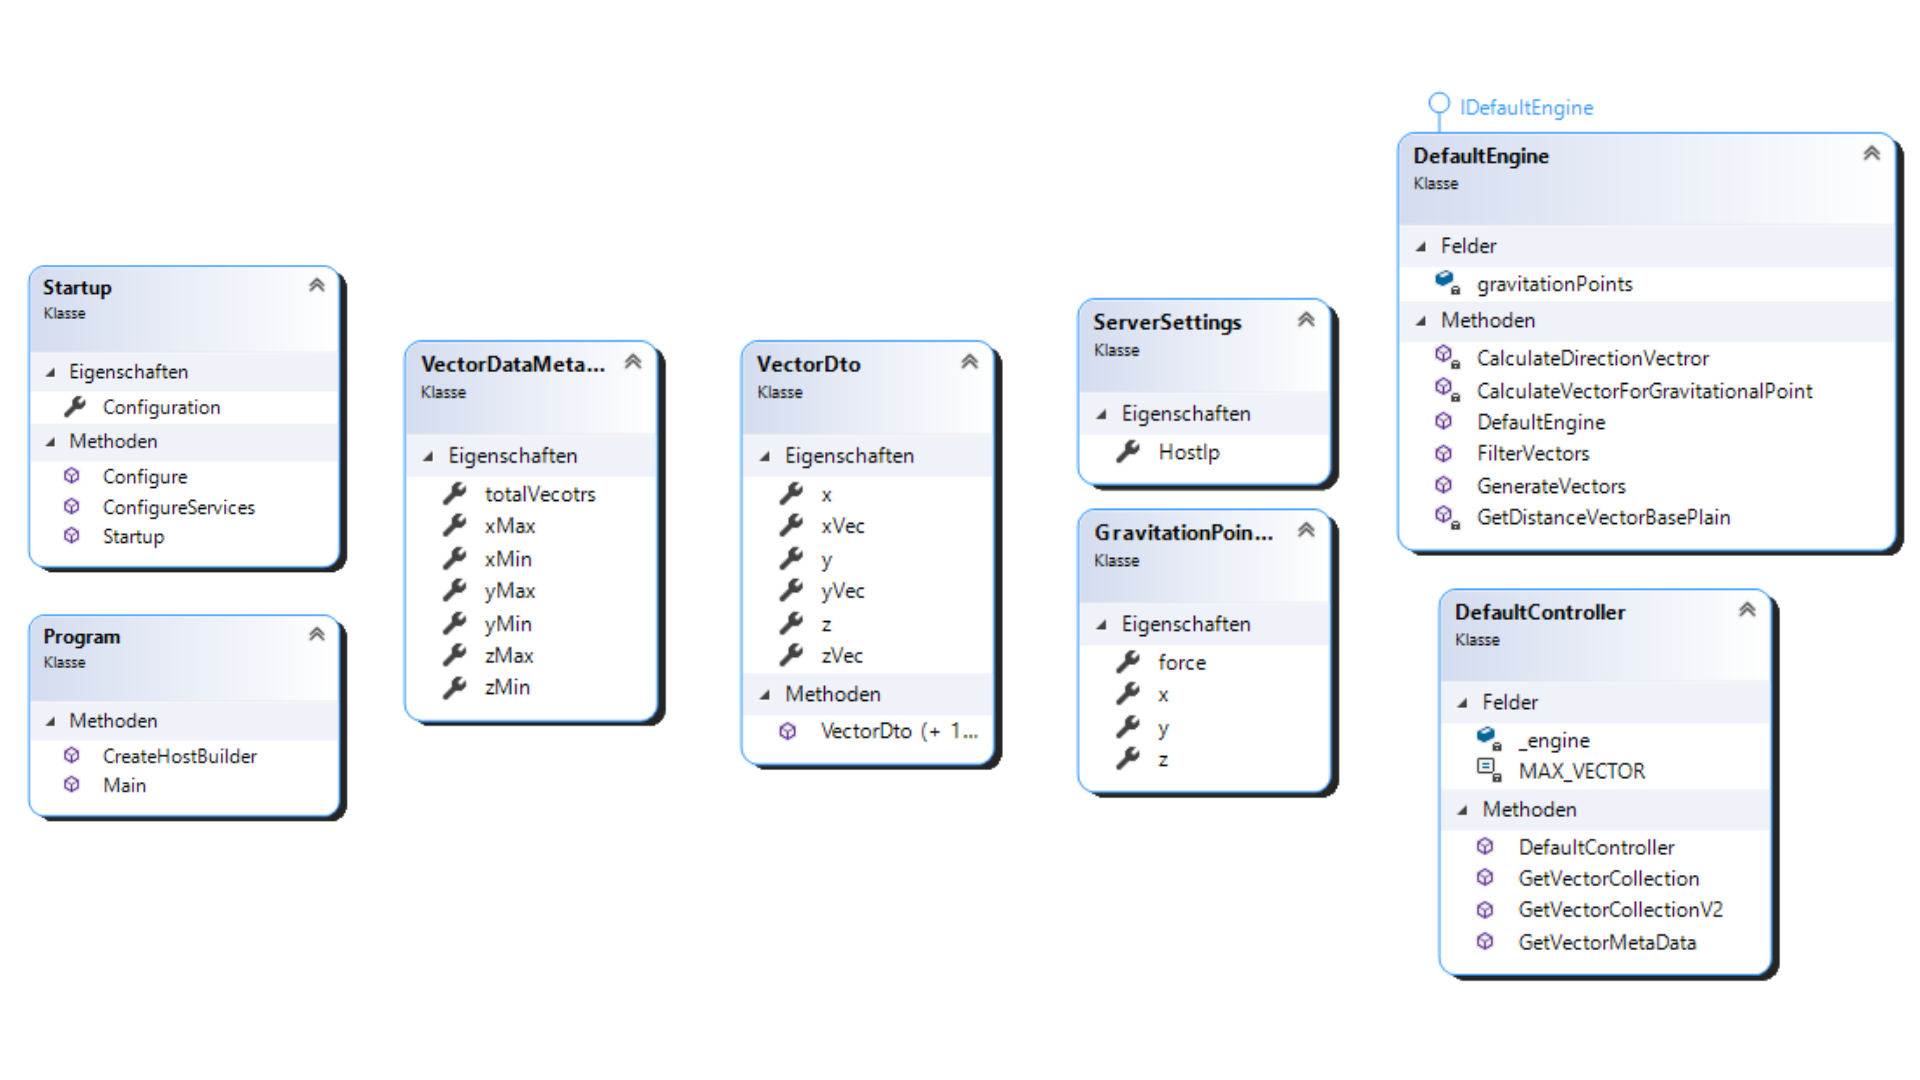
\includegraphics[width=\linewidth]{images/backend/classDiagram}
	\caption{System Klassen, Dto Klassen und Controller und Engine Klassen}
	\label{fig:ClassDiagram}
\end{figure}

Die Backend API wird in Asp.NetCore (C\#) implementiert. Das Framework wurde gewählt, da es kostenlos und opensource ist und da es sowohl auf Linux als auch auf Windows lauffähig ist (vgl. DotNet Download page \cite{DotNetDownloadPage}). Außerdem liefert NetCore mit ASP nativ eine IIS Webapplikation Funktionalität mit, sodass die API schnell und einfach umzusetzen ist, ohne einen großen web hosting Overhead zu erzeugen. Grundsätzlich besteht das Programm aus drei Klassen Gruppen, den System Klassen, den Controller und Engine Klassen und den Daten Transfer Objekt (Dto) Klassen (siehe Abbildung \ref{fig:ClassDiagram}).\\
Die Klasse Programm besitzt vordefinierten code zur Instanziierung des WebHosts. Um Die Host Ip selbst festlegen zu können wurde dieser code um die ServerSettings erweitert, welche die HostIp aus der apsettings.json bezieht (Code \ref{codefig:Program.cs}:7) und im CreateHostBuilder diese als HostURL verwendet (Code \ref{codefig:Program.cs}:16).\\
\begin{codefig}
	\centering
	\lstset{style=sharpc}
	\begin{lstlisting}
public static void Main(string[] args)
{
	var config = new ConfigurationBuilder()
		.AddJsonFile("appsettings.json", optional: false)
		.Build();
	var serSet = new ServerSettings();
	config.GetSection("ServerSettings").Bind(serSet);
	CreateHostBuilder(args, serSet).Build().Run();
}

public static IHostBuilder CreateHostBuilder(string[] args, ServerSettings serverSettings) =>
	Host.CreateDefaultBuilder(args)
		.ConfigureWebHostDefaults(webBuilder =>
		{
			webBuilder.UseStartup<Startup>();
			webBuilder.UseUrls(serverSettings.HostIp);
		});
	\end{lstlisting}
	\caption{Methoden der Program Klasse}
	\label{codefig:Program.cs}
\end{codefig}
In der zweiten Systemklassen \grqq Startup.cs\grqq\space werden die Webhost und Umgebungseinstellungen getätigt. In Code \ref{codefig:ConfigureServices} Zeile 3 wird der Teil \grqq AppSettings\grqq\space aus der \grqq appsettings.json\grqq\space ausgelesen und in die Dto Klasse \grqq AppSettings\grqq\space geparsed. Diese Instanz wird dann mithilfe von Dependency injection an alle Instanzen verteilt, welche das Objekt benötigen. In den Zeilen 4 - 8 wird für später die CORS Policy definiert. Die hier definierte Policy wird jede Origin, mit jeder HTTP Methode und jedem Header akzeptieren. Außerdem wird in Zeile 9 eine Instanz von DefaultEngineV2 als Singleton für IDefaultEngine via Dependancy Injection definiert. Dependency Injection wird verwendet um ein einfaches austauschen der Engine zu ermöglichen und zur Vereinfachung des Lifetimemanagement der DefaultEngineV2 Instanz im DefaultController.\\
\begin{codefig}
	\centering
	\lstset{style=sharpc}
	\begin{lstlisting}
public void ConfigureServices(IServiceCollection services)
{
	services.Configure<AppSettings>(Configuration.GetSection("AppSettings"));	
	services.AddCors(o => o.AddPolicy("AllowAnyOrigin", builder => {
		builder.AllowAnyOrigin()
			.AllowAnyMethod()
			.AllowAnyHeader();
	}));
	services.AddSingleton<IDefaultEngine, DefaultEngineV2>();
	services.AddControllers();
	services.AddDirectoryBrowser();
}
	\end{lstlisting}
	\caption{Methode ConfigureServices in Startup.cs}
	\label{codefig:ConfigureServices}
\end{codefig}
Diese Methode wird zu Laufzeit vor Configure (Code \ref{codefig:Configure}) aufgerufen. In Configure werden nun einige wichtige Einstellungen getätigt. In Code \ref{codefig:Configure} Zeile 3 wird die vorher in ConfigureServices definierte \grqq AllowAnyOrigin\grqq -Policy für die ganze WebApp übernommen. In den Zeilen 11 - 17 wird eingestellt welche statischen Dateien gehostet werden sollen, wo diese liegen und wo diese aufzufinden sein sollen. So wird nun der gesamte Inhalt des Ordners wwwroot am /data Endpunkt zur Verfügung gestellt. Der zuvor erstellte FileExtensionContentTypeProvider (Code \ref{codefig:Configure}: 5 - 9) definiert mit welchem Content-Type Header die "unbekannten" Datentypen übermittelt werden sollen. Wenn keine eindeutige Definition vorliegt wird die Datei mit dem Standard Header "text/html" nur dann ausgeliefert wenn ServeUnknowFileTypes auf true gesetzt wurde.
Asp.NetCore liefert von sich einen Directory Browser mit, welcher eine graphische UI zur Navigation durch die statischen Dateien generiert (siehe Abbildung \ref{fig:DirectoryBrowser}). Dieser wird in Zeile 18 aktiviert. Die letzten Zeilen sind von Asp.NetCore für API Anwendungen standardmäßig generierte Codezeilen. Sie aktivieren das Standard Routing und definieren die Controller als verarbeitende Endpunkte.\\
\begin{codefig}
	\centering
	\lstset{style=sharpc}
	\begin{lstlisting}
public void Configure(IApplicationBuilder app, IWebHostEnvironment env)
{
	app.UseCors("AllowAnyOrigin");

	var provider = new FileExtensionContentTypeProvider();
	provider.Mappings[".dat"] = "application/octet-stream";
	provider.Mappings[".patt"] = "text/html";
	provider.Mappings[".mtl"] = "text/html";
	provider.Mappings[".obj"] = "text/html";

	app.UseStaticFiles(new StaticFileOptions
	{
		ServeUnknownFileTypes=true,
		FileProvider = new PhysicalFileProvider(Path.Combine(env.WebRootPath, "data")),
		RequestPath = "/data",
		ContentTypeProvider = provider
	});
	app.UseDirectoryBrowser();
	app.UseRouting();
	app.UseEndpoints(endpoints =>
	{
		endpoints.MapControllers();
	});
}
	\end{lstlisting}
	\caption{Methode Configure in Startup.cs}
	\label{codefig:Configure}
\end{codefig}

\begin{figure}
	\centering
	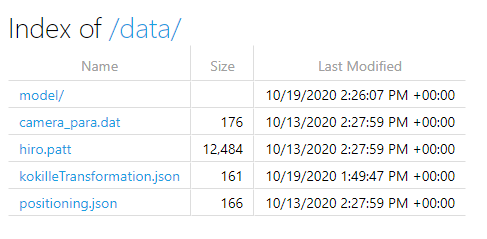
\includegraphics[width=0.7\linewidth]{images/backend/DirectoryBrowser}
	\caption{Directory Browser zur Navigation durch statische Dateien des Servers}
	\label{fig:DirectoryBrowser}
\end{figure}

Bei der ersten anfrage an die API wird eine Instanz des implementierten Controllers erstellt, welche nun die einkommenden Anfragen verarbeitet. Der DefaultControler bekommt bei Instanziierung via Dependency Injection die vorher in ConfigureServices definierte Instanz einer IDefaultEngine Interface implementierenden Klasse (vgl. Code \ref{codefig:DefaultControllerConstructor}). Diese Aufteilung in Controller und Engine wurde definiert um eine besser Codeübersicht zu gewährleisten. So ist die input verarbeitende Controller Klasse von der Datenverarbeitenden Engine Klasse losgelöst.

\begin{codefig}
	\centering
	\lstset{style=sharpc}
	\begin{lstlisting}
private IDefaultEngine _engine;

public DefaultController(IDefaultEngine engine)
{
	_engine = engine;
}
	\end{lstlisting}
	\caption{Konstruktor der DefaultController Klasse}
	\label{codefig:DefaultControllerConstructor}
\end{codefig}

Die Controller Klasse implementiert die in Kapitel 2.3 Definierten Endpunkte. GetVectorMetaData bezieht die Metadaten mit einem Methoden Aufruf aus der Engine Klasse und gibt diese dann zurück.
Die GetVectorCollection Methode akzeptiert 8 optionale Parameter (siehe Tabelle \ref{tab:EndpointQueryParameters}). Aufgrund von API design best practices (vgl. Narumoto \cite{ApiDesignBestPractices}) und aufgrund von potentiell hoher Datenmenge unterstützt der Endpunkt pagination. Durch setzen von limit und offset kann so gesteuert werden wieviele und welche Teile der Vektor Daten zurückgegeben werden. Durch angeben von n1, n2, n3, x, y, und z können die Ergebnisse zusätzlich gefiltert werden. Dies geschieht in der Engine Klasse.
\begin{table}
	\centering
	\begin{tabular}[h]{p{0.11\linewidth} | p{0.7\linewidth}| p{0.09\linewidth}}
	Parameter & Beschreibung & Default \\
	\hline
	limit & Limitiert die Anzahl an zurückgegebenen Vectoren & 100\\
	offset & Definiert den Abstand vom ersten zurückgegebenen Vektor zum ersten Vektor im Datensatz & 0\\
	n1 & x-Koordinate des Normalenvektors der Filter-Ebene & null\\
	n2 & y-Koordinate des Normalenvektors der Filter-Ebene & null\\
	n3 & z-Koordinate des Normalenvektors der Filter-Ebene & null\\
	x & x-Koordinate eines punktes auf der Filter-Ebene & null\\
	y & y-Koordinate eines punktes auf der Filter-Ebene & null\\
	z & z-Koordinate eines punktes auf der Filter-Ebene & null\\
	maxDist & Definiert den maximalen Abstand, den ein Punkt von der Filter-Ebene haben darf um zurückgegeben zu werden & 0.5\\
	\end{tabular}
	\caption{Query Parameter des api/data/ Endpunktes}
	\label{tab:EndpointQueryParameters}
\end{table}
Die DefaultEngine Klasse Implementiert, das IDefaultEngine Interface und mit Ihr auch die Methoden GetAllVectors, GetVectorMetaData, und FilterVectors. Sie bezieht die AppSettings des Programms via Dependency Injection (vgl. Code \ref{codefig:DefaultEngineConstructor}).
\begin{codefig}
	\centering
	\lstset{style=sharpc}
	\begin{lstlisting}
private AppSettings _settings;

public DefaultEngineV2(IOptions<AppSettings> settings)
{
	_settings = settings.Value;
}
	\end{lstlisting}
	\caption{Konstruktor der DefaultEngine Klasse}
	\label{codefig:DefaultEngineConstructor}
\end{codefig}
Dieses Settings Objekt ist erforderlich, da es den Pfad zu der Datei beinhaltet, welche die Vektordaten enthält. Dieser Pfad wird von der Methode \grqq GetAllVectors\grqq\space an die private Methode \grqq LoadVectorsFromJsonFile\grqq\space weitergegeben, welche wiederrum mithilfe des \grqq StreamReaders\grqq\space zunächst die datei einliest und ansachließend mit \grqq JsonConvert\grqq\space in eine Liste an VectorDto objekten parst. (vgl. Code \ref{codefig:GetAllVectors})
\begin{codefig}
	\centering
	\lstset{style=sharpc}
	\begin{lstlisting}
private List<VectorDto> LoadVectorsFromJsonFile(string path)
{
	var returnList = new List<VectorDto>();

	using (StreamReader r = new StreamReader(path))
	{
		string json = r.ReadToEnd();
		returnList = JsonConvert.DeserializeObject<List<VectorDto>>(json);
	}

		return returnList;
	}

public List<VectorDto> GetAllVectors()
{
	return LoadVectorsFromJsonFile(_settings.jsonPath);
}
	\end{lstlisting}
	\caption{Akquirieren der Vektordaten von einer in den App-Settings definierten Datei}
	\label{codefig:GetAllVectors}
\end{codefig}
Diese Funktionen werden auch von \grqq GetVectorMetaData\grqq\space aufgerufen, welche dann jeweils die x,y und z minima und maxima und die Anzahl an Vektoren ermittelt ermittelt. Diese werden dann als \grqq VectorDataMetaData\grqq\space zurückgegeben.\\
Die Engine Klasse stellt auch eine FilterVectors Methode zur Verfügung. Die Methode nimmt einen ein plainVectorDto Objekt, die maximale Distanz und die zu filternden Vektoren entgegen. Um die Distanz von einem Punkt zu einer Ebene zu ermitteln muss zunächst die Ebene in Koordinatenform ($n1 \cdot x + n2 \cdot y + n3 \cdot z = c$) angegeben werden können. Hierführ muss nurnoch c ermittelt werden, was durch einsetzen der werte errechnet werden kann. Anschließend wird für jeden punkt die Distanz mit der Formel $d = \frac{n1 \cdot x + n2 \cdot y + n3 \cdot z - c}{\sqrt{n1^2 + n2^2 + n3^2}}$. Diese Distanz wird mit der maximalen Distanz verglichen und der Vektor wird nur dann zurückgegeben, wenn diese kleiner oder gleich ist (vgl. Code \ref{codefig:FilterVectors}).
\begin{codefig}
	\centering
	\lstset{style=sharpc}
	\begin{lstlisting}
private double GetDistanceVectorBasePlain(double n1, double n2, double n3, double c, VectorDto vector)
{
	return Math.Abs(n1 * vector.x + n2 * vector.y + n3 * vector.z - c) / Math.Sqrt(Math.Pow(n1, 2) + Math.Pow(n2, 2) + Math.Pow(n3, 2));
}

public List<VectorDto> FilterVectors(List<VectorDto> vectors, VectorDto plainVector, double maxDist)
{
	double n1 = plainVector.xVec;
	double n2 = plainVector.yVec;
	double n3 = plainVector.zVec;

	double px = plainVector.x;
	double py = plainVector.y;
	double pz = plainVector.z;

	double c = n1 * px + n2 * py + n3 * pz;

	return vectors.Where((v) => GetDistanceVectorBasePlain(n1, n2, n3, c, v) <= maxDist).ToList();
}
	\end{lstlisting}
	\caption{Filtern der Vektoren anhand der Distanz von einer Filterebene}
	\label{codefig:FilterVectors}
\end{codefig}
Während der Entwicklung, waren zunächst keine Daten verfügbar. Daher wurden die Vektordaten ursprünglich durch ein Gravitation Modell simuliert. Auf diese Simulation wird in der Arbeit nicht weiter eingegangen.\\
Das Backend wurde mit der Vektordaten Simulierung zu Testzwecken während der Entwicklung in einem Azure Webservice gehostet.

%\begin{itemize}
%	\item Framework: Netcore (C\#)
%	\begin{itemize}
%		\item Ausgewählt da
%		\item NetCore sowohl auf Linux alsauch Windows verfügbar
%		\item ASP Netcore eine stabile und aktuelle grundlage für WebApplications und WebAPIs bietet (liefert viele funktionen nativ mit)
%	\end{itemize}
%	
%	\item Klassendiagramm
%	\begin{itemize}
%		\item Einzelne Klassen beschreiben
%	\end{itemize}
%		
%	\item CORS
%	\begin{itemize}
%		\item Implementierung:
%		\begin{itemize}
%			\item Hinzufügen einer Policy in Netcore, welche alle Origins erlaubt
%		\end{itemize}
%	\end{itemize}
%	
%	\item Implementierung der Endpunkte
%	\begin{itemize}
%		\item Daten auslieferung/gewinnung
%		\begin{itemize}
%			\item Simulation der daten früher via Gravitationsmodell
%			\item Simulation jetzt durch ausliefern vorberechneter und vorgegebener Simulationsdaten
%		\end{itemize}
%				
%		\item Filterung
%		\item Meta Info auslieferung
%	\end{itemize}
%		
%	\item Ausliefern der statischen daten und aufbereitung mit DirecotryBrowser durch NetCore mitgelieferten funktionen
%	\begin{itemize}	
%		\item Hinzufügen eines FileExtensionContentTypeProvider für nicht nativ unterstützte Dateien (.dat, .patt, .mtl, .obj)
%	\end{itemize}
%		
%	\item Hosten in Azure zu entwicklungszwecken
%\end{itemize}



	\section{Schlussfolgerung und Ausblick}

\begin{itemize}
	\item Vorgaben nicht umsetzbar ohne abstriche.
	\item AR.js läuft besser auf handy als auf PC
	\item Visualisierung is eig kake - Microsof MX wär doch viel geiler
	\item Direkter Informationstransport zwischen kokille und backend muss umgesetzt werden (aktuell ja nur simulations daten)
	\item HTTPS hosting in lokaler umgebung aufesetzbar
	\begin{itemize} \renewcommand{\labelitemii}{$\Rightarrow$}
		\item Gerät muss zertifikat vertrauen
	\end{itemize}
	
	\item Andere implementierung des Backends
	\begin{itemize}
		\item Kann für Visualisierung in anderen Feldern helfen
		\begin{itemize}
			\item z. B. Luftströme bei Autos, etc.
		\end{itemize}
	\end{itemize}
\end{itemize}

% Needed so build won't break (as long as no other citations exist)
Dummy text\cite{MetamorphicTesting}.

	
	\section*{Arbeitsteilung}

\newcommand{\by}[1]{\hfill\textsl{#1}}


\subsection*{Textuelle Ausarbeitung}

\begin{enumerate}[label*=\arabic*.]
	\item \textbf{Einleitung} \by{Michael Mican}
	
	\item \textbf{Methodik}
	
	\begin{enumerate}[label*=\arabic*.]
		\item Allgemeiner Aufbau
		
		\begin{enumerate}[label*=\arabic*.]
			\item Projekt Vorgaben \by{Michael Mican}
			\item Probleme und Abweichungen von den Vorgaben \by{Michael Mican}
			\item Komponenten \by{Maximilian Seitz}
		\end{enumerate}
		
		\item Visualisierung/Frontend \by{Maximilian Seitz}
		
		\item Daten Bereitstellung/Backend \by{Michael Mican}
	\end{enumerate}
	
	\item \textbf{Ergebnisse}
	
	\begin{enumerate}[label*=\arabic*.]
		\item Implementierung des Frontends \by{Maximilian Seitz}
		
		\item Implementierung des Backends \by{Michael Mican}
	\end{enumerate}
	
	\item \textbf{Schlussfolgerung und Ausblick} \by{Maximilian Seitz}
\end{enumerate}


\subsection*{Programmatische Ausarbeitung}

\begin{itemize}
	\item \textbf{Frontend} \by{Maximilian Seitz}
	
	\begin{itemize}
		\item GUI (für Einstellungen) \by{Michael Mican}
	\end{itemize}
	
	\item \textbf{Backend} \by{Michael Mican}
\end{itemize}

	
	%\lstlistoflistings
	
	\pagebreak
	\bibliography{bib}
\end{document}



